\section{Identical-Pool Selection}
\label{sec:identical-pool}
\label{sec:search-vs-selection}

\subsection{Does trace-conditioned selection beat identical-pool consensus?}

Table~\ref{tab:main-matrix}'s Class~B columns and Figure~\ref{fig:pooled4} test whether
failure-trace gated deferral (FTA) adds value beyond plurality when candidate availability is held
fixed. FTA and Pooled-4 operate on the same four-generator answers, so their paired difference
isolates the commit rule rather than discovery. On that shared pool ($n{=}3394$; 15 cells),
Pooled-4 accuracy is $66.53\%$ ($2258/3394$) and FTA is $65.00\%$ ($2206/3394$): $-1.53$\,pp for FTA
(McNemar $p{=}0.00027$; discordant FTA/Pooled-4/tie counts $73/125/3196$). A stratified within-cell
paired bootstrap ($10{,}000$ replicates) places the Pooled-4$-$FTA gap at $+1.53$\,pp with 95\%
percentile interval $[+0.74,\,+2.33]$\,pp; the gap remains positive under leave-one-provider,
leave-one-dataset, and leave-one-cell deletion. Omitting Azure reduces the gap to $+0.52$\,pp
(McNemar $p{=}0.30$), so the aggregate advantage is concentrated but directionally stable.
Descriptively, Pooled-4 matches or exceeds FTA in $13/15$ completed cells (most per-cell gaps are
within resampling noise; bootstrap replicates reproduce $\geq 13/15$ only $\approx 17\%$ of the
time). FTA is strictly higher only on Vertex$\times$MATH-500 and Vertex$\times$GPQA. A unique
plurality exists on $88\%$ of examples; the $12\%$ Frontier-fallback subset is harder ($26\%$ vs.\
$74\%$ accuracy). Alternative deterministic tie rules move overall accuracy by at most
$\sim\!1.3$ points (\ref{app:compute-detail}).

\begin{figure}[tbp]
\centering
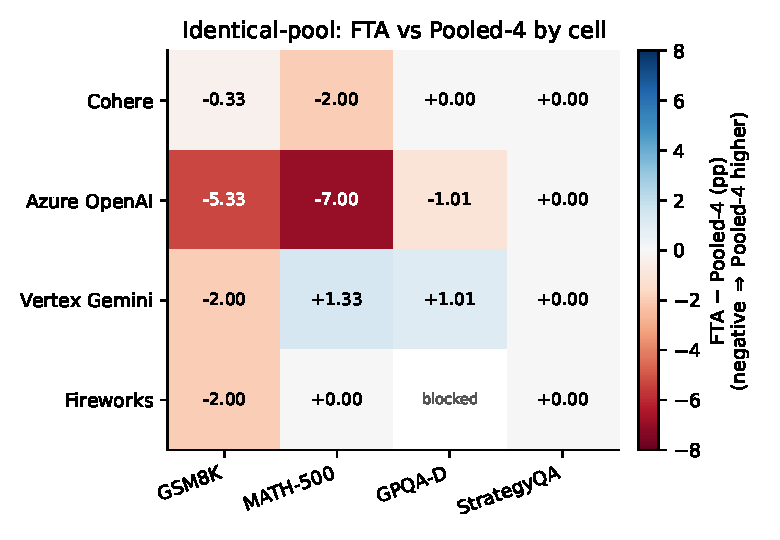
\includegraphics[width=0.78\linewidth]{figure5_fta_vs_pooled4_delta_heatmap}
\caption{Per-cell difference in accuracy (FTA$-$Pooled-4, percentage points) on the \emph{identical}
four-generator pool. Negative values favor plurality. The comparison holds candidate availability
fixed, so the map isolates commit-rule effects. Fireworks$\times$GPQA is protocol-blocked.}
\label{fig:pooled4}
\end{figure}

Positive consensus regret $\mathrm{CR}(\mathrm{FTA})$ (Section~\ref{sec:problem}) means this
failure-derived rule extracts less accuracy from the shared pool than plurality. Without that
control, occasional FTA gains over a single Class~A generator could be misread as selection progress.
The measurement point is attribution: once candidate availability is fixed, this commit rule has
positive consensus regret despite some generator-relative gains.

\subsection{When FTA differs from its Class~A generator, is the pattern transfer?}

Relative to Frontier alone, FTA improves in $8/15$ cells, regresses in $6/15$, and ties in $1/15$.
After Holm-corrected paired McNemar tests, supported gains appear in four cells and supported
regressions in two (Azure$\times$GSM8K, Azure$\times$MATH-500). Figure~\ref{fig:heatmap} treats that
heterogeneity as transfer evidence for the commit rule.

\begin{figure}[tbp]
\centering
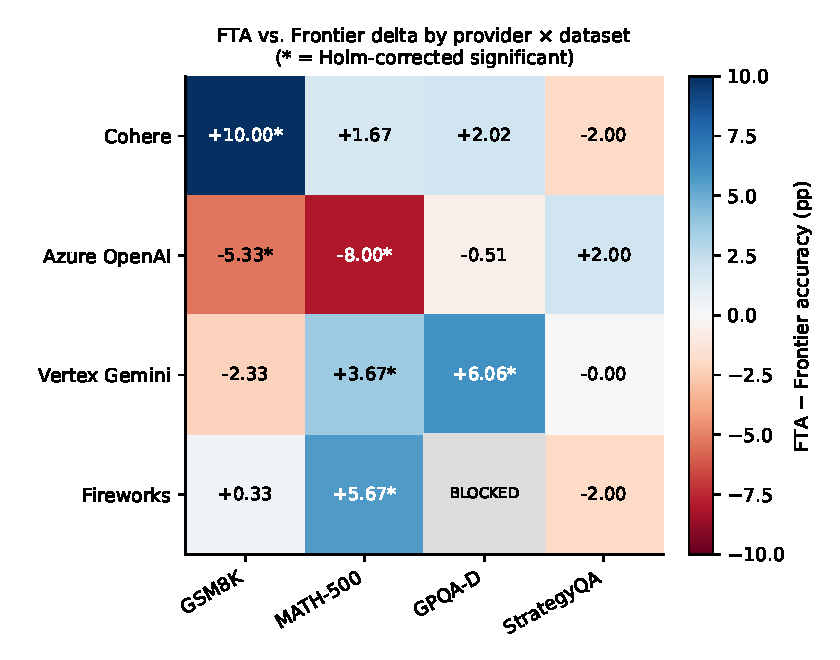
\includegraphics[width=0.74\linewidth]{figure2_fta_frontier_delta_heatmap}
\caption{Per-cell FTA$-$Frontier accuracy delta. Asterisks mark Holm-corrected supported
differences. Signs vary by provider; Azure has the only negative provider mean---transfer evidence
for the commit rule, not a uniform selector ranking.}
\label{fig:heatmap}
\end{figure}

\paragraph{Diagnostic cells}
\textbf{Cohere$\times$GSM8K} (Tier~A; development-adjacent): high discovery ($0.907$); FTA improves
over Frontier yet trails Pooled-4 slightly. \textbf{Azure$\times$GSM8K}: discovery near ceiling
($0.927$) with FTA harming both Frontier and Pooled-4---selection failure under high discovery.
\textbf{Vertex versus Azure GPQA:} matched discovery ($\approx 0.636$) with opposite FTA signs.
StrategyQA ($n{=}100$) effects are near zero and are not treated as strong evidence.

\subsection{Can cell-level selection improve over a fixed policy without leakage?}
\label{sec:heldout-calibrated-selector}

We ask whether a leakage-free selector calibrated only on training cells can choose among a frozen
method set for a held-out provider--dataset cell. The design uses leave-one-cell-out over the $15$
completed cells; candidate methods are Frontier, FTA, the L1-/S1-/TALE-style adapters, and Pooled-4;
features are coarse cell-level summaries (provider, dataset, and training-only empirical
accuracies). The preregistered protocol hash is shown in two lines:
{\footnotesize\ttfamily
9d1978ffcd3211d62476ceb11a3e8eae\par
06dc8d5d8c073336a9d60bf3c7724257\par}
An earlier non-leakage-free analysis is excluded.

\begin{table}[tbp]
\centering
\footnotesize
\setlength{\tabcolsep}{4pt}
\caption{Leave-one-cell-out selector over $15$ completed cells with coarse cell-level features.
The selector chooses Pooled-4 in every fold and ties fixed Pooled-4; the oracle row is
non-deployable headroom.}
\label{tab:heldout-selector-phase8}
% Validated from the leakage-free held-out selector cell-level results.
\begin{tabularx}{\textwidth}{@{}Yrrrrc@{}}
\toprule
Policy & Correct & Total & Accuracy & Deploy. & Outcome use \\
\midrule
Held-out learned policy & 2258 & 3394 & 66.53\% & Yes & No \\
Best training-selected fixed method & 2258 & 3394 & 66.53\% & Yes & No \\
Fixed Pooled-4 & 2258 & 3394 & 66.53\% & Yes & No \\
Frontier & 2176 & 3394 & 64.11\% & Yes & No \\
FTA replay selector & 2206 & 3394 & 65.00\% & Yes & No \\
Oracle cell selector & 2287 & 3394 & 67.38\% & No & Yes \\
\bottomrule
\end{tabularx}

\end{table}

Table~\ref{tab:heldout-selector-phase8} gives the full result. Within this $15$-cell design and
feature set, the leakage-free selector does not improve over fixed Pooled-4.
